%% An example of the article based on superfri.cls class file of
%% ``Supercomputing Frontiers and Innovations. An International Journal''
%% http://superfri.org/.

\RequirePackage{fix-cm}

\documentclass{superfri}
\usepackage[hidelinks]{hyperref}
\usepackage{lmodern}% http://ctan.org/pkg/lm
\usepackage{algorithm}
\usepackage{algpseudocode}

%\usepackage{nicefrac}
%\usepackage{mathtools}
%\usepackage{tabularx,booktabs,ragged2e}
%\usepackage{xcolor}
%\usepackage{showframe}
\usepackage[framemethod=tikz]{mdframed}

% ------------

\bibliographystyle{superfri}
\begin{document}

\author{Roman Kaplan\footnotemark \and Leonid Yavits\footnotemark[\value{footnote}] \and Ran Ginosar\footnotemark[\value{footnote}]}
\footnotetext[1]{Israel Institute of Technology, Haifa, Israel}

\title{SuperFri article template}

\maketitle{}

\begin{abstract}

\keywords{Content Addressable Memory, Associative Processing, in-storage processing, memristors}
\end{abstract}

% -----------------------------------------------------------------------
\section*{Abstract}
\label{sec:abstract}
Near-data in-memory processing research has been gaining momentum in recent years. Typical processing-in-memory architecture places a single or several processing elements next to a volatile memory, enabling processing without transferring data to the host CPU. The processing elements benefit from an increased bandwidth to and from the volatile memory. Since this approach does not place processing next to the lowest hierarchy in the von Neumann architecture, i.e., in storage, it is exposed to the problems faced by von Neumann architectures, namely the bandwidth wall. 

The goal of this work is to design a storage device that does not suffer from the von Neumann bandwidth bottleneck and can provide high performance on massively parallel workloads. To achieve this, a novel processing-in-storage system based on Resistive Content Addressable Memory (ReCAM) is presented. ReCAM functions simultaneously as storage and as a parallel associative processor. ReCAM processing-in-storage resolves the bandwidth wall by keeping computation inside the storage array, thus implementing in-data, rather than near-data, processing. 

This work shows that ReCAM based processing-in-storage architecture may outperform existing processing-in-memory and accelerator based designs. ReCAM processing-in-storage implementation of Smith-Waterman DNA sequence alignment reaches a speedup of almost five over a GPU cluster. An implementation of in-storage inline data deduplication is presented and shown to achieve orders of magnitude higher throughput than traditional CPU and DRAM based systems.

\section{Introduction}
\label{sec:motivation}
Until the breakdown of Dennard scaling designers focused on improving performance for a single core by increasing its clock rate. Since 2005, when Dennard scaling diminished but Moore's law continued, the focus has shifted to increasing the number of cores in multicore processors \cite{esmaeilzadeh2011dark}. Increasing the number of cores allowed to reduce processing time. However, data transfer time did not improve at the same rate, making memory-CPU bandwidth a main bottleneck of performance.

Data is typically fetched to the CPUs and their memory hierarchies from non-volatile storage such as hard disks or Flash SSDs. Consequently, bandwidth and access-time to storage pose a major constraint to improve performance. The throughput at which data can be fetched from storage to the processing units (CPU or an accelerator) has become a main determinant of system performance. The problem worsens in a datacenter cloud environment, where a dataset can be distributed among multiple nodes across the datacenter. In this case, communicating the stored data adds latency and reduces bandwidth even further, placing low bounds for maximal performance.

This challenge has motivated re-emerging Near-Data Processing (NDP) \cite{balasubramonian2014near}. The data-centric NDP shifts computing closer to data. NDP seeks to minimize data movement by computing at the most appropriate location in the hierarchy, which can be cache, main memory or persistent storage. With NDP, less data needs to be transferred through levels of hierarchy, thus alleviating the limited bandwidth problem. NDP proposals that place computing resources at the cache level \cite{yavits2015computer} or in main memory \cite{guo2011resistive}\cite{ahn2015scalable}\cite{de2016cudalign} (also known as Processing-in-Memory or PiM) do not address the bandwidth bottleneck problem facing workloads with large datasets (or big data). In-storage NDP targets the source of the problem, but offers only a partial solution.

Resistive CAM (ReCAM), a storage device based on emerging resistive materials in the bitcell with a novel non-von Neumann Processing-in-Storage (PRinS) compute paradigm, is proposed in order to mitigate the storage bandwidth bottleneck of big data processing. Section \ref{sec:background} provides background on the basic concepts of ReCAM and PRinS and covers related work. Section \ref{sec:PRinS_with_ReCAM} presents the ReCAM architecture, explains how processing is performed within ReCAM and establishes its scalability. PRinS implementations of two algorithms are presented in Sections \ref{sec:smith_waterman} and \ref{sec:dedup} and compared to other approaches: Smith-Waterman DNA sequence alignment and in-storage data deduplication.


\section{Background and Related Work}
\label{sec:backgroud}
Three basic concepts underline the proposed ReCAM: content addressable memories, associative processing and resistive materials. The following two subsections introduce each concept. The third subsection covers related work on NDP and highlights their limitations at addressing the storage bandwidth challenge of big data processing.

\subsection{Content Addressable Memory and Associative Processing}
\label{sec:CAMandAP}
Content addressable memory (CAM), also called associative memory, allows the comparison of all data words to a key in parallel, tagging the matching words, and possibly reading some or all of the tagged words, one by one. Standard memory read and write operations of a single word at a time can also take place.
In addition to storing information, a CAM array can be modified to function as an associative processor \cite{foster1976content}\cite{yavits2015resistive}. In associative processing, the parallel compare and parallel write operations supported by CAM are used to implement an ‘if condition then value' expression. Thus, complex Boolean expressions are evaluated in parallel on all data words (CAM rows) by sequential execution of truth table if-then lines. Each (multi-bit) argument of a truth table line is matched with the contents of the appropriate field in the entire CAM array: the matching rows are tagged and the corresponding result values from the truth table line are written into the designated fields of all tagged rows. 
For an $m$-bit argument $x$, any Boolean $f(x)$ has $2^m$ possible values, therefore the associative computing operation should incur $O(2^m)$ cycles, regardless of the dataset size. More efficiently, arithmetic operations can be performed on ReCAM in a word-parallel, bit-serial manner, reducing compute time from $O(2^m)$ to $O(m)$. The massive parallelism of each operation compensates in performance for the relatively large number of (parallel execution) cycles of each arithmetic operation.
More complex computations (more than Boolean functions) are decomposed into series of Boolean expressions, as usual [41][43]. 

\subsection{Resistive Memories}
\label{sec:resistive_memories}
Resistive memories store information by modu-lating the resistance of nanoscale storage elements (memristors). Memristors are two-terminal devices, where the resistance of the device is changed by the electrical current or voltage. The resistance of the memristor is bounded by a minimum resistance $R_{on}$ (low resistive state, logic '1') and a $R_{off}$ maximum resistance (high resistive state, logic '0').

Resistive memories are non-volatile, free of leakage power, and emerge as long-term potential alternatives to charge-based memories, including NAND flash. The metal-oxide resistive random access memory (ReRAM), employing one resistive device and possibly also one transistor (1R1T) per bit-cell, is considered a potential technology to replace next-generation nonvolatile memories. Its main features are high reliability and fast access speed. A test-chip of 32GB device with two ReRAM-based memory layers and a CMOS logic layer underneath has been developed \cite{ahn2015pim}, demonstrating design techniques to achieve a high density functional chip. 

\subsection{Related Work}
\label{sec:related_work}
%The concept of NDP has been considered for several decades \cite{kogge1999short}. One approach to implementing NDP employs 3D stacked memories (e.g., \cite{ahn2015scalable}\cite{giridhar2013exploring}). DRAM memory is placed on top of a logic die allowing for a high-speed vertical inner interface between the memory and logic. The Hybrid Memory Cube \cite{liu2014swaphi} is another memory design (and a product) that exploits the increased bandwidth between DRAM and near-memory logic, and may be exploited for NDP \cite{azarkhish2017logic}. 


<Start of in vs. near-data>

%% 2D CMOS PiM 
%\subsubsection{2D Processing-in-Memory Architectures}
%\label{sec:2D_PiM}
While processing-in-storage research is relatively young, the wider concept of near-data processing, focusing mainly on processing in memory (PIM) has been thoroughly researched. The concept of mixing memory and logic has been around since 1960s. The DAPP, STARAN, CM-2, and GAPP computer architectures \cite{potter1989array} used large number of processing units positioned in proximity to memory arrays to implement a massively parallel SIMD computer. Gokhale et al. [31] designed TeraSys, a computer architecture comprising a conventional host processor where at least part of its memory was replaced by a PIM array, integrating memory and ALUs in close proximity. Hall et al. [37] developed DIVA, the Data-Intensive Architecture, combining PIM memories with external host processors and performing selected computations in processing elements near memory and reducing the volume of data transferred across the long and slow processor-memory interface. Kogge et al. [41] developed HTMT, a parallel multilevel memory architecture, where each RAM level is a PIM memory (memory blocks interconnected with ALUs). Suh et al. [68]  introduced a SLIIC QL computer featuring a processor integrated on the same die as DRAM. Lipovsky et al. 46] developed a dynamic associative access memory architecture that combined DRAM and a single-bit processing element, capable of associative and conventional arithmetic processing, placed in the sense amplifier area of a DRAM. Yavits et al. [56] suggested replacing the last level cache and the vector co-processor of a conventional high-performance CPU by an associative processor, which is a PIM accelerator, combining data storage and massively parallel SIMD processing capabilities. Nitin et al. [70] introduced RowCore, a near-memory processing architecture for Big Data Machine Learning. Gao et al. [30] proposed Heterogeneous Reconfigurable Logic, a reconfigurable array for near-data processing systems.

%% 3D CMOS PiM 
\subsubsection{3D Processing-in-Memory Architectures}
\label{sec:3D_PiM}
While embedding processing with conventional 2D DRAM chips is less practical, recent advancement in 3D memory and logic stacking technology may remove this obstacle. Citing severe bandwidth limitations in conventional computer architecture as datasets continue to grow, Ahn et al. [1] introduced Tesseract, a 3D Processing in Memory accelerator for large-scale graph processing. In another work, Ahn et al. [2] developed a hybrid memory cube based framework that automatically decides whether to execute PIM operations in memory or processors depending on the locality of data. Nair, Sura et al. [69][53] introduced the Active Memory Cube, a heterogeneous computing system including general-purpose host processors and specially designed in-memory processors that would be integrated in a logic layer within 3D DRAM memory. In another work, Gao et al. [52] developed hardware and software of a 3D stack memory and near-data processing architecture for in-memory analytics frameworks, including MapReduce, graph processing, and deep neural networks. Azarkhish et al. [7] developed Smart Memory Cube and designed a high bandwidth interconnect to serve the bandwidth demand of PIM architecture. Zhang et al. [76] explored PIM implemented via 3D die stacking. Akin et al. [3] addressed the issue of data reorganization in 3D stacked near-data processing architecture, introducing HAMLeT, a mechanism for host interference, bandwidth allocation, and in-memory coherence. Farmahini-Farahani et al. [27] proposed NDA, a near-DRAM acceleration architecture that processes data using accelerators 3D-stacked on DRAM devices.

%% Resistive PiM 
\subsubsection{Processing-in-Memory with Resistive Materials}
\label{sec:Resistive_PiM}
Recently, emerging memory technologies such as resistive memory have become a focus of PIM research. Somnath et al. ‎[59] developed MBARC, a resistive crossbar in-memory LUT-based processing architecture. Chi et al. ‎[16] introduced PRIME, a PIM accelerator of neural network applications in RRAM based main memory. ‎[57] introduced a resistive CAM based massively parallel accelerator. Shafiee et al. [65] developed an in-situ processing architecture, where memristor crossbar arrays are used to perform dot-product operations in an analog manner. 

%% Near-data PRinS
\subsubsection{Near-Data Processing-in-Storage}
\label{sec:NDP_PRinS}
Flash-based SSD allowed for increased in-storage bandwidth, enabling data port from each chip thus achieving higher data throughput. Typical processing-in-storage architecture places a single or several processing cores inside the storage and allows data processing without transferring it to the host processor. The concept of near-data processing-in-storage is illustrated in Figure \ref{fig:in_vs_near_data}a. 

\begin{figure}[h!]
	\centerline{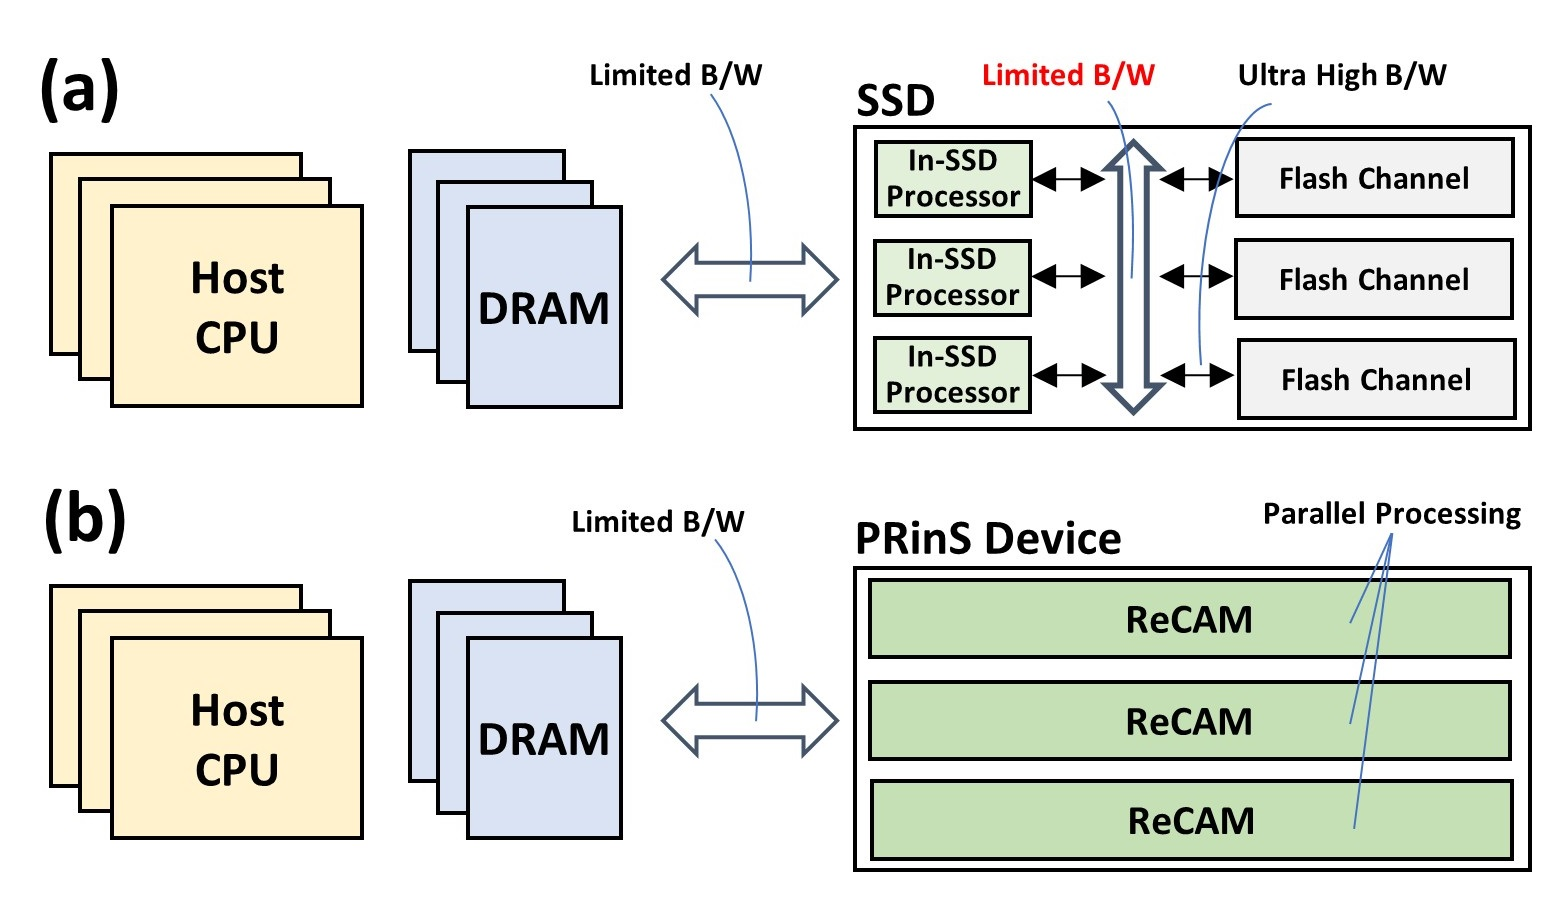
\includegraphics{Figures/In_vs_near_data.jpg}}
	\caption{Comparison of (a) \textbf{near-data} processing-in-storage (b) and \textbf{in-data} processing-in-storage based on ReCAM.}
	\label{fig:in_vs_near_data}
\end{figure}


Boboila et al. [12] proposed Active Flash, a processing in solid-state storage that expedites data analysis by migrating the data to the flash device. The authors explored energy and performance trade-offs of their processing-in-storage architecture. Bae et al. [8] introduced the notion of Intelligent SSDs, exploring the design considerations and examining their potential benefits in data mining applications. Continuing the work on Intelligent SSD, Jo et al. [38] studied optimal ways of combining CPU, GPU and SSD for efficient processing of data-intensive algorithms. Cho et al. [17] cited the lack of parallel processing abilities in earlier in-SSD processing architectures and proposed integrating a GPU, providing API sets based on the MapReduce framework. Kang et al. [40] introduced the Smart SSD model, which combines in-SSD processing with a powerful host system, and constructed a Smart SSD prototype. De et al. [22] introduced the FPGA-based Minerva, which executed application-specific operations in the NVM controller. Jun et al. [39] introduced and constructed BlueDBM, combining a flash based storage with in-store processing capability and a low latency high-throughput inter-controller network, and explored its performance benefits. Cho et al. [18] explored some of the questions which are also addressed by this paper. The authors made a case for Intelligent SSD by discussing the bandwidth trends and quantifying the potential benefits of processing-in-storage across a range of applications.

<End of in vs. near-data>

\section{Processing-in-Storage with ReCAM}
\label{sec:PRinS_with_ReCAM}

The approach of this work is to design a device for storing big datasets and processing them efficiently. The key properties of this design are scalability and massively parallel processing, possible due to the non-von Neumann architecture. Parallelism is achieved by in-situ processing of the data, in contrast with NDP approaches. In this work, Resistive CAM (ReCAM), a non-volatile and scalable storage device with resistive bitcells and a novel Processing-in-Storage (PRinS) paradigm is presented. The concept is demonstrated in Figure \ref{fig:in_vs_near_data}b.

\subsection{ReCAM Crossbar Array}
\label{sec:ReCAM_crossbar}
While ReRAM may employ one transistor and one memristor (1T1R) cells, ReCAM uses 2T2R cells, following \cite{akinaga2010resistive}\cite{azarkhish2017logic}. Figure \ref{fig:ReCAM_IC} shows the resistive CAM crossbar. A bitcell, shown in Figure \ref{fig:ReCAM_IC}a, consists of two transistors and two resistive elements (2T2R). The KEY register contains a data word to be written or compared against. The MASK register defines the active columns for write and read operations, enabling bit selectivity. The TAG register (Figure \ref{fig:ReCAM_IC}b) marks the rows that are matched by the compare operation and may be affected by a parallel write. The TAG register enables chaining multiple ReCAM ICs.
In a conventional CAM, compare operation is typically followed by a read of the matched data word. When in-storage processing involves arithmetic operations, a compare is usually followed by a parallel write into the unmasked bits of all tagged rows, and additional capabilities, such as read and reduction operations, are included \cite{yavits2015resistive}. 

\tab{tab:recam_operations}{Operations included in ReCAM}{
	\begin{tabular}{cc}
	\hline
	Integer Instruction (32bit) $\quad $ & $\quad $ Cycles \\
	\hline
	B $\leftarrow$ A+B & $\quad $256 \\
	C $\leftarrow$ A+B & $\quad $512 \\
	Shift down by one row & $\quad $96 \\
	Row-wise Max (A,B) & $\quad $64 \\
	Max Scalar (A) & $\quad $64 \\
	\hline
	\end{tabular}
}

Any computational expression can be efficiently implemented in ReCAM storage using line-by-line execution of the truth table of the expression \cite{balasubramonian2014near}. Arithmetic operations are typically performed bit-serially. Table \tabref{tab:recam_operations} lists several operations supported by ReCAM and the number of cycles required by each operation.  Shifting down a consecutive block of rows by one row position requires three cycles per bit. First, compare-to-‘1' copies the source bit-column of all rows into the TAG. Second, shift moves the TAG vector down by setting the shift-select line (Figure 1b). Third, write-'1' copies the shifted TAG to the same bit-column. Shifting 32-bit numbers thus requires 96 cycles. Addition (in-place or not) is performed in a bit-serial manner using a truth table approach \cite{balasubramonian2014near} (32 bits times 8 truth-table rows times 2 for compare and write amount to 512 cycles). Row-wise maximum compares in parallel two 32-bit numbers in each row. Max Scalar tags all rows that contain the maximal value in the selected element. Additional operations, such as parallel and reduction arithmetic, may be required for other algorithms. 



\begin{figure}[h!]
	\centerline{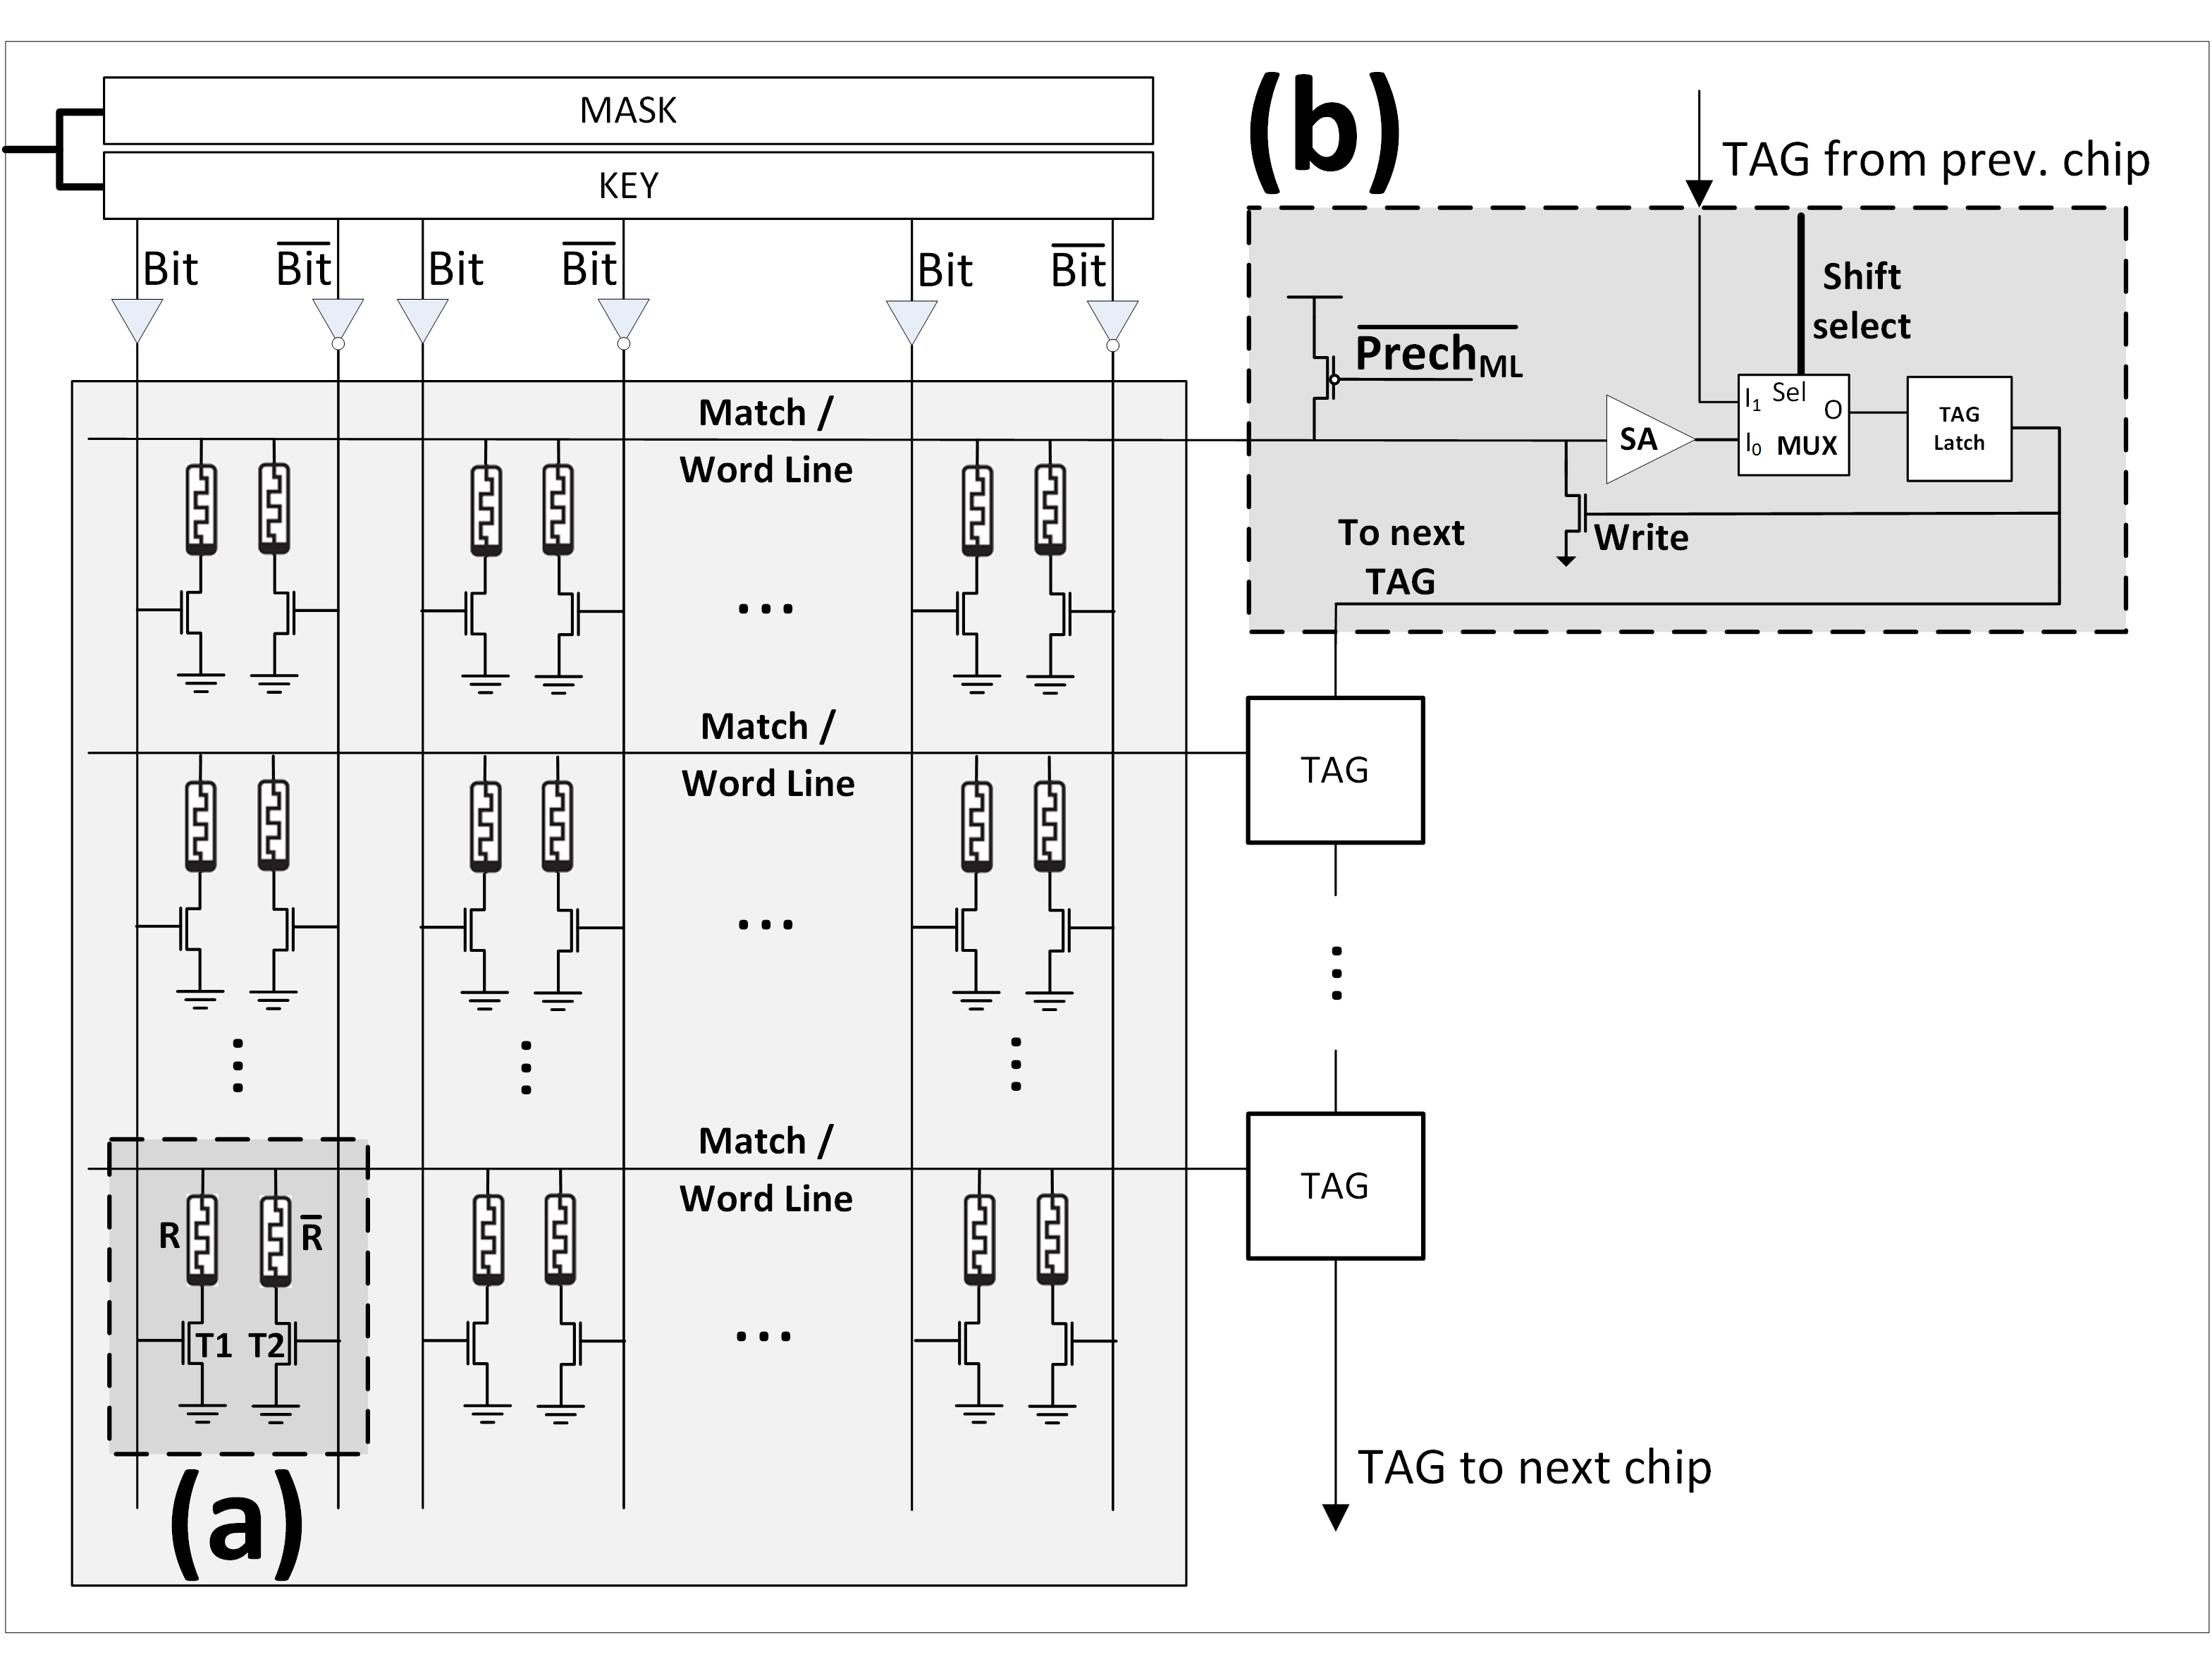
\includegraphics[scale=0.4]{Figures/ReCAM_array.jpg}}
	\caption{Single ReCAM crossbar integrated circuit. (a) 2T2R ReCAM bitcell. (b) TAG logic.}
	\label{fig:ReCAM_IC}
\end{figure}




\subsection{System Architecture}
\label{sec:system_architecture}
Conceptually, the ReCAM comprises hundreds of millions of rows, each serving as a computational unit. Due to power die restrictions, the entire array may be divided into multiple smaller ICs, as in Figure \ref{fig:ReCAM_IC}a. A row is fully contained within an IC. All ICs are daisy chained for Shift and Max Scalar operations.
The ReCAM storage system uses a microcontroller (Figure \ref{fig:ReCAM_IC}b) similar to \cite{guo2013ac}. It issues instructions, sets the KEY and MASK registers, handles control sequences and executes read requests. In addition, the microcontroller may also perform some baseline processing, such as normalization of the reduction tree results.
ReCAM-based storage is scalable due to its inherent parallelism. It allows for scalability by adding more ICs and increasing storage capacity at no performance cost since compute capability is linearly scalable in the number of ICs. Therefore, processing in-storage of large data sets does not require ReCAM for external communication, in contrast to datacenter-scale storage. 

\begin{figure}[h!]
	\centerline{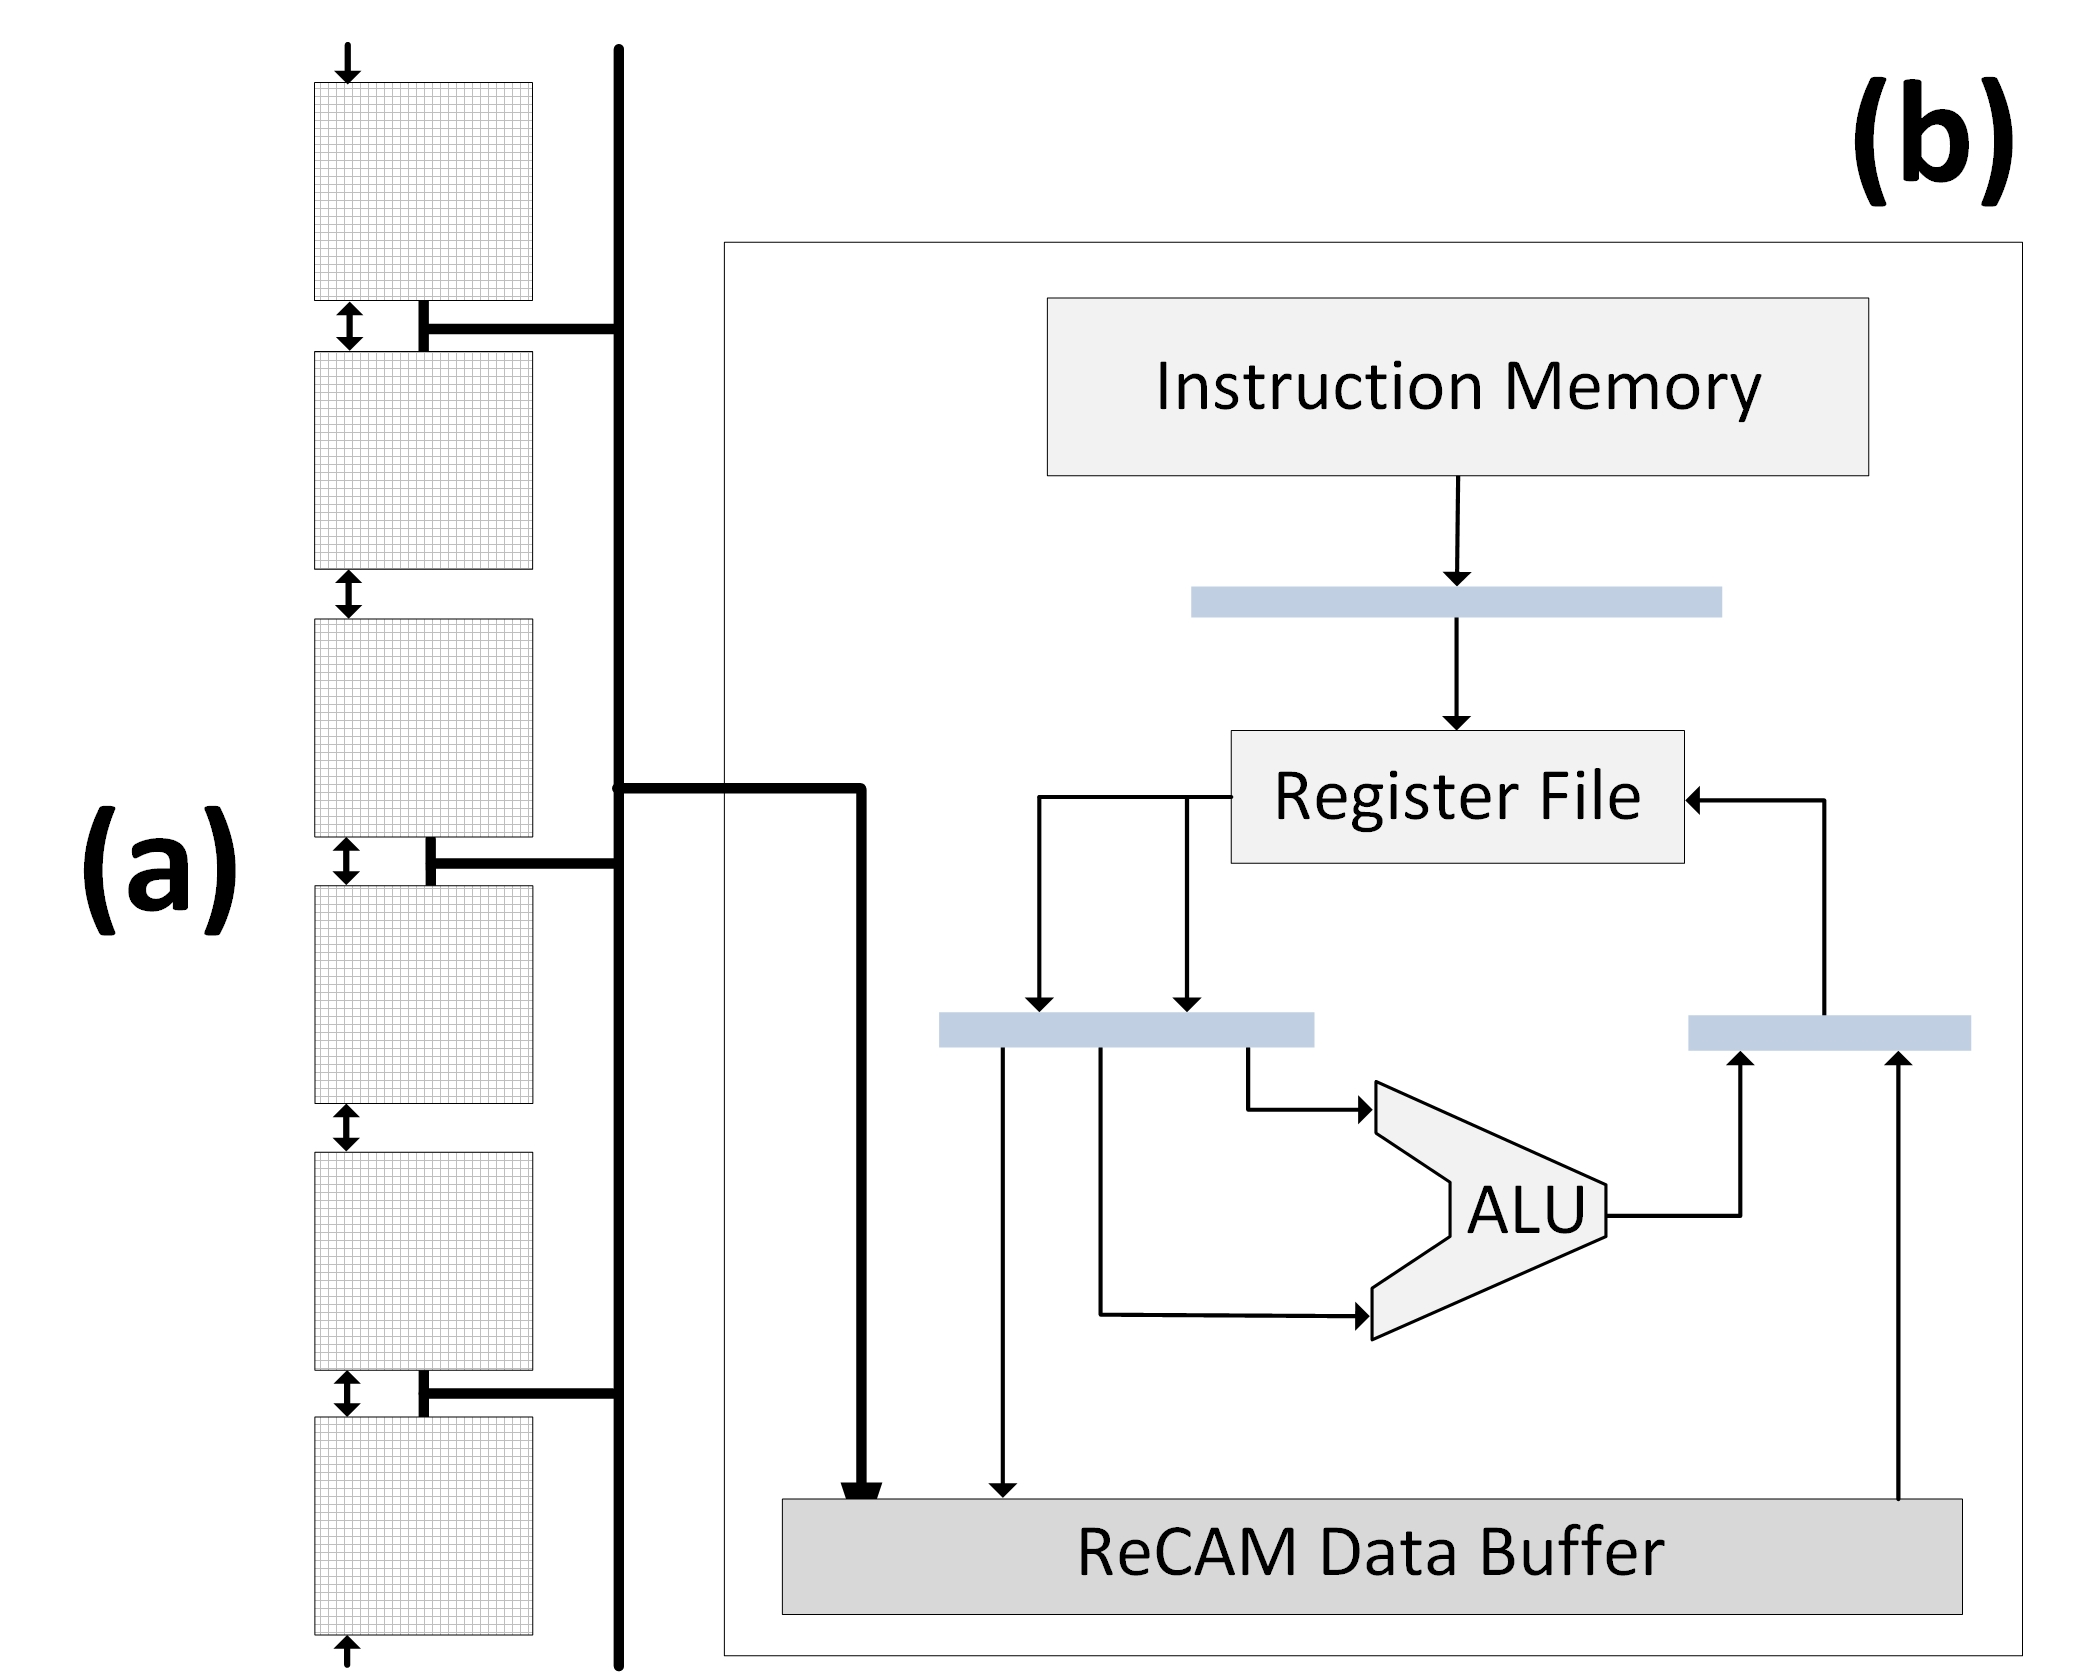
\includegraphics[scale=0.6]{Figures/ReCAM_Single_IC_Column.jpg}}
	\caption{Complete ReCAM-based Storage system, composed of (a) separate multiple daisy-chained ICs and (b) Microcontroller. Connected to the multiple ICs with a reduction tree network.}
	\label{fig:ReCAM_system}
\end{figure}

\section{PRinS Application: Smith-Waterman DNA Sequence Alignment}
\label{sec:smith_waterman}

Searching for similarities in pairs of protein and DNA sequences (also called Pairwise Alignment) has become a routine procedure in Molecular Biology and it is a crucial operation in many bioinformatic tools. The Smith-Waterman algorithm (S-W) \cite{smith1981identification} provides an optimal solution for the pairwise sequence alignment problem, but requires a number of operations proportional to the product of the two sequences. 
S-W identifies the optimal alignment of two sequences by computing a two-dimensional scoring matrix. Matchings base-pairs score positively, while mismatching result in a negative score. The optimal alignment score of two sequences is the highest score in the matrix. The S-W has two steps: scoring (to find the maximal alignment score) and trace-back to construct the alignment. The first step is the most computationally demanding and is the focus of this work.

\begin{figure}[h!]
	\centerline{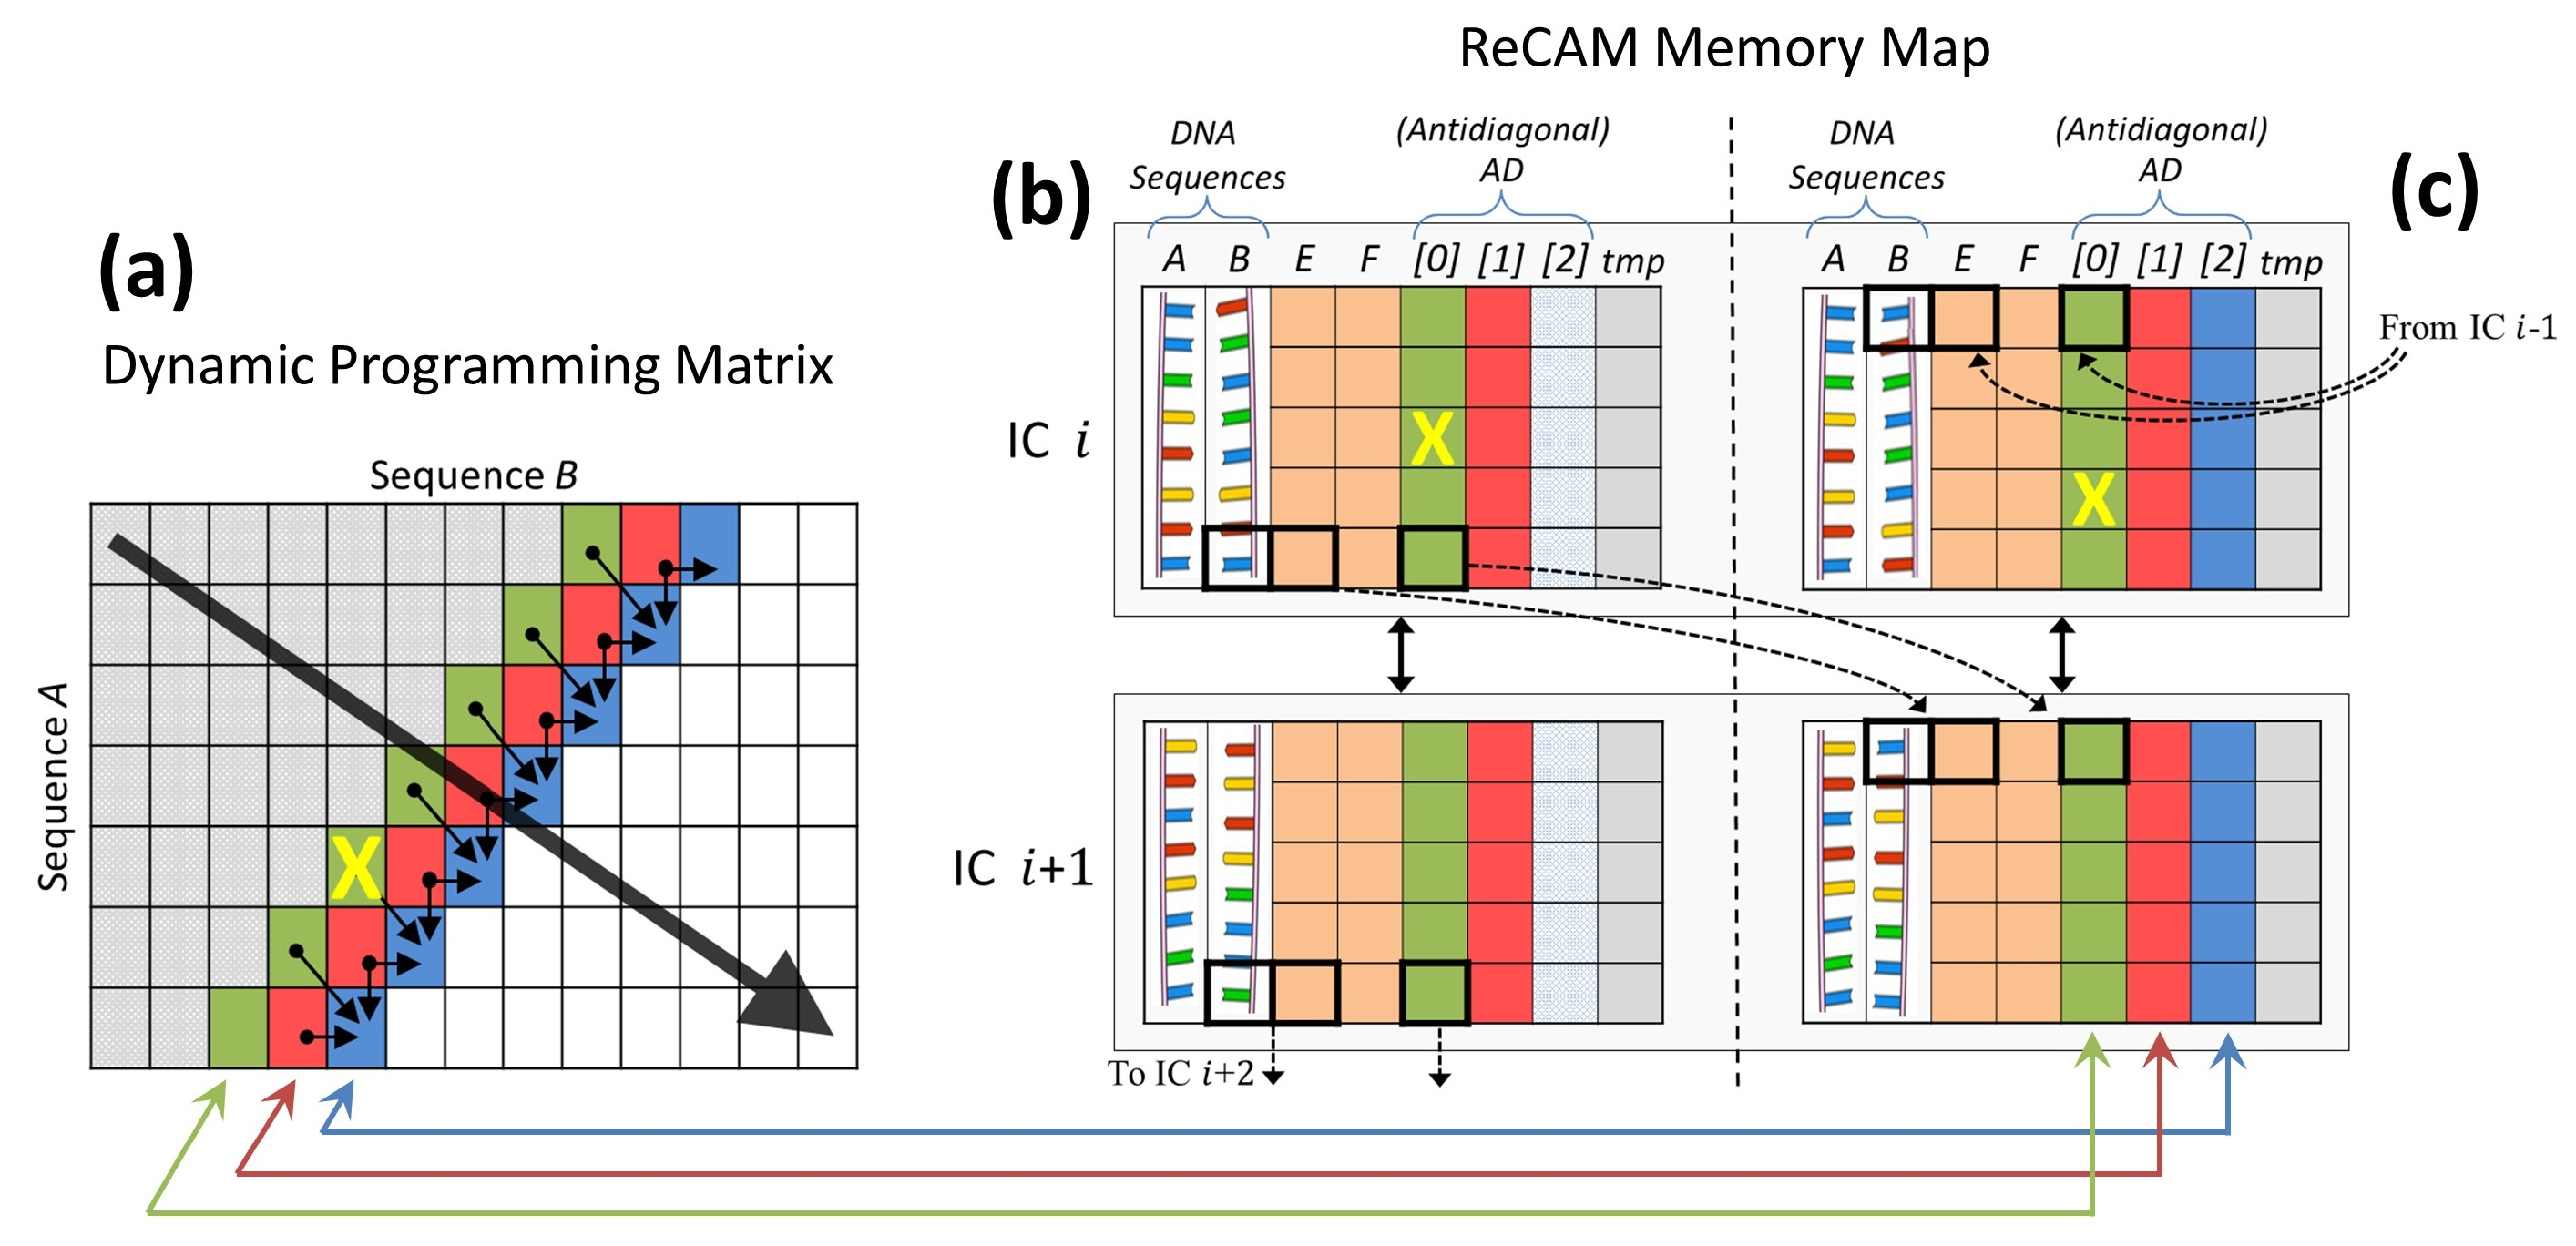
\includegraphics[scale=0.6]{Figures/SW_on_ReCAM_Figure.jpg}}
	\caption{Mapping the dynamic programming matrix on ReCAM. (a) A snapshot of the dynamic programming matrix, shows the direction of progress for the parallel algorithm. (b) and (c) shows an example of organization of data in the ReCAM crossbar array at the beginning (b) and end (c) of an iteration. AD[2] contents in (b) is being replaced with the new result (c). Bottom rows in a crossbar IC are daisy-chained to the next IC in a shift instruction. The cell marked with X contains the global maxmium score.}
	\label{fig:SWonReCAM}
\end{figure}

Figure \ref{fig:SWonReCAM}a shows a snapshot of the scoring matrix during the algorithm execution. In a parallel implementation, the matrix is filled along the main diagonal and the entire anti-diagonal scores are calculated in parallel. Figure \ref{fig:SWonReCAM}b shows the ReCAM memory map of two consecutive ICs at the beginning of an iteration. A and B contain the sequences, where each base-pair takes 2-bit and resides in a separate row. E and F are partial score results of the affine gap model \cite{giridhar2013exploring}. AD[0], AD[1] and AD[2] contain scoring matrix anti-diagonals. Scores are represented by 32-bit integers. Shift operations in the PRinS implementation move data between rows inside an IC and between daisy-chained ICs. Figure \ref{fig:SWonReCAM}c shows the ReCAM memory map at the end of an iteration and the mapping between ReCAM and the scoring matrix. A complete description of the S-W PRinS implementation appears in \cite{kaplan2017resistive}.

\subsection{simulation and comparison to state-of-the-art}
\label{sec:SW_simulation}

\tab{tab-mytable}{Simulated ReCAM parameters}{
	\begin{tabular}{cc}
		\hline
		ReCAM Parameter$\quad $ & $\quad $Value \\
		\hline
		Active storage size$\quad $ & $\quad $8GB\\
		Frequency$\quad $ & $\quad $1Ghz \\
		Power per integrated circuit$\quad $ & $\quad $200W \\
		Number of integrated circuit$\quad $ & $\quad $32 \\	
		\hline
	\end{tabular}
}

A cycle-accurate simulator of the ReCAM storage was constructed. Assumed operational frequency is 1GHz. An in-house power simulator was used to evaluate the power consumption of ReCAM. The latency and energy figures used by both the timing and power simulations are obtained using SPICE simulation and are detailed in \cite{yavits2015resistive}. 

We simulate the ReCAM with the cycle-accurate simulator. Assumed ReCAM parameters are listed in Table <X>. The CUPS metric (Cell Updates per Second) is used to measure S-W performance. Results are compared to other works in Table 2. The in-storage implementation is compared to other implementations in different platforms: a 384-GPU cluster \cite{de2016cudalign}, the 128-FPGA RIVYERA platform \cite{wienbrandt2014fpga} and a four Xeon Phi implementation \cite{liu2014swaphi}. On ReCAM with a total of 8GB in 32 separate ICs, each 256MB and 8M rows, 53 TCUPS are demonstrated, computing a total of $57\times10^{12}$ scores. $4.7\times$ faster than the best implementation. The table also shows computed GCUPS/Watt ratios; ReCAM is close to twice better than the FPGA solution and $80\times$ better than the GPU system.



\tab{tab-mytable}{Summary of state-of-the-art performance for S-W scoring step in previous works and in ReCAM}{
	\begin{tabular}{ccccc}
	\hline
	Accelerator & Xeon Phi & FPGA & GPU & ReCAM\\
	\hline
	Performance (TCUPS) & 0.23 & 6.0 & 11.1 & 53\\
	Number of ICs & 4 & 128 & 384 & 32 \\
	Power (kWatt) & 0.8 & 1.3 & 100 & 6.6  \\
	GCUPS/Watt & 0.3 & 4.7 & 0.1 & 8.0 \\	
	Reference & \cite{liu2014swaphi} & \cite{wienbrandt2014fpga} & \cite{de2016cudalign} &  \\	
	\hline
	\end{tabular}
}


\section{PRinS Application: In-Storage Data Deduplication}
\label{sec:dedup}
Deduplication is a data compression technique for eliminating redundant copies of repeated data, designed to improve storage utilization. Files are split into multiple data blocks. Only unique blocks are meant to be stored. With every new write, a data block is compared against all blocks in the storage. If a match occurs, a pointer to the previously stored block is saved in lieu of the data block. Given that the same data block may occur multiple times (match frequency is also dependent on the block size), storage efficiency can be greatly improved \cite{zhu2008avoiding}.

Deduplication operates on the physical layer of the storage, managing a set of data structures to expose a consecutive logical layer of storage. Each data block has two addresses, physical (PA) and logical (LBA). Only the LBAs are exposed to the outside world, while physical addresses are used internally by the deduplication mechanism.

\subsection{Related Work: Conventional Deduplication}

\begin{figure}[ht!]
	\centerline{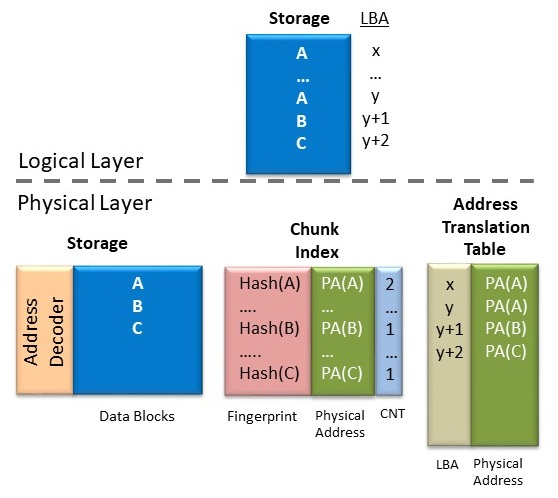
\includegraphics[scale=0.6]{Figures/dedup_PC.jpg}}
	\caption{Conventional deduplication scheme after writing the following sequence of (data block, LBA): (A, x), (A, y), (B, y+1), (C, y+2). The storage, chunk index and address translation table reside in the physical layer.}
	\label{fig:dedup_PC}
\end{figure}

In a typical inline storage deduplication system (comprising disk / SSD storage, CPU and DRAM for holding indices and tables), the basic deduplication data unit is termed a chunk. Upon writing a new data chunk to storage, comparing the chunk contents (typically 4-8 KByte) to the entire storage is infeasible. Instead, a much shorter representation, called a fingerprint or hash (e.g., 20-byte SHA-1 hash) is calculated for each chunk, and the fingerprint is looked up in a chunk index. If no entry is found, the chunk is stored and a new entry is added to the chunk index. In addition to the fingerprint, the index entry also holds at least the chunk's PA and the number of references to it (Figure 18). If the fingerprint of the new chunk is found, its number of references is incremented. An additional address translation table holds both the LBA and the PA of each chunk.

Conventional implementations of deduplication require a dedicated computer within the storage appliance. For example, a disk-based deduplication system \cite{zhu2008avoiding} with usable capacity of 6TB employs 15 SATA drives (connected in RAID6), 500GB each, and two dual-core CPUs with 8GB of DRAM. It reaches 90\% CPU utilization at peak I/O performance. All chunk metadata is stored on disk, while the DRAM serves as a cache for chunk metadata, to reduce non-I/O storage access. An expansion of that system \cite{debnath2010chunkstash} includes a flash-based SSD serving as fast storage for the entire chunk metadata. The configuration is similar to \cite{zhu2008avoiding}, although smaller, with a RAID4 storage comprising five hard drives, 500GB each, a dual-core CPU and 4GB of DRAM. As in the previous work, DRAM serves as a small cache for chunk metadata.  Xtremio's X-brick \cite{XbrickSpec} is an example of an all-flash high-end large-scale contemporary storage appliance. Each of its units contains either 13 or 25 SSDs with an effective capacity of 3.2 or 7.2 TB, respectively. The appliance supports up to 8 units and uses a quad-core processor with 256GB of DRAM. 

At the other end of the spectrum, \cite{chen2011caftl} shows an example of an in-SSD deduplication with the purpose of enhancing the device endurance. The authors suggest using the device controller and memory buffer to calculate the chunk fingerprint. Deduplication is implemented with an additional indirection in the flash translation layer and uses the buffer as a small cache (similar to the DRAM in \cite{debnath2010chunkstash} and \cite{zhu2008avoiding}). 


\subsection{In-Storage ReCAM Based Deduplication}

\begin{figure}[ht!]
	\centerline{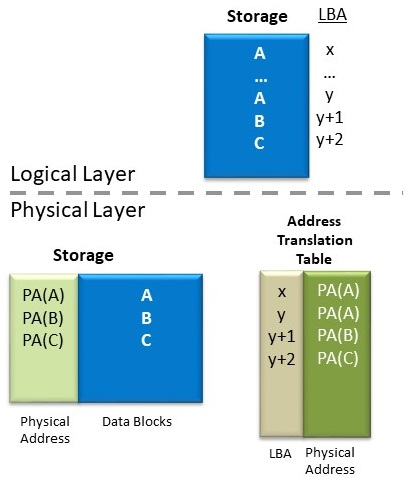
\includegraphics[scale=0.6]{Figures/dedup_ReCAM.jpg}}
	\caption{ReCAM based deduplication scheme, following the same sequence of writes as in Figure \ref{fig:dedup_PC}.}
	\label{fig:dedup_ReCAM}
\end{figure}

The proposed ReCAM based inline deduplication requires neither external CPU nor DRAM. The deduplication is accomplished entirely within the ReCAM, using its in-storage processing capabilities. ReCAM based deduplication is illustrated in Figure 19. Each data block in ReCAM storage is divided into $S=(block\_size)⁄(ReCAM\_width)$ row-segments of $ReCAM\_width$ size. For example, for 256-bit wide ReCAM and 4KB blocks, the number of segments is $S=128$. Data blocks are stored in ReCAM in segment by segment fashion, in $S$ consecutive ReCAM rows. The first segment of each data block is marked by '1' in the block\_start bit column. The values of $block\_start$ in all other ReCAM rows of the data block are zero. 

Otherwise, the new block is unique. In that case it is written into the ReCAM along with its (arbitrarily assigned, unique) PA. As described above, the block is written segment by segment into $S$ consecutive rows, and the first segment is marked '1' in the start\_block bit column. 

In both cases (unique and duplicate), the LBA of the data block is placed together with its PA in an associative address translation table, which can be stored in a separate module of the ReCAM storage. The translation table mapping can be optimized to eliminate storing multiple copies of the same PA (of duplicated blocks). Overall, write takes $O(S)$ cycles.  

Read is done in two steps. First, the LBA of the data block is searched in the associative address translation table. The corresponding PA is retrieved from the table. Second, the PA is searched in the ReCAM storage (by compare), followed by read of the data block from the matched ReCAM rows. It is accomplished by a series of S read operations, starting with the row marked by '1' in the start\_block bit column. Overall, read operation takes $O(S)$ cycles.  
 
Deletion of a data block is performed in three steps. In the first step, the LBA is searched in the address translation table; its PA is retrieved (to be used at the second step), and the entry at the address translation table is deleted (using the delete\_data function of Figure 17). In the second step, the PA (retrieved at the first step) is searched again in the address translation table; if MATCH returns '0', it means that the deleted block has no duplicates. In this case, it is deleted from the ReCAM storage, in $O(S)$ cycles.

A complete description of the in-storage deduplication appears in \cite{kaplan2016deduplication}.  


\begin{figure}[!ht]
	%\begin{algorithm}[H]
		%\caption{Associative Write, Read and Delete in ReCAM-based data deduplication}
		%\label{array-sum}
		
		\begin{mdframed}[
			linecolor=black,
			linewidth=1pt,
			roundcorner=2pt,
			backgroundcolor=white,
			userdefinedwidth=\textwidth,
			]
		\begin{algorithmic}[1]
			\Function{Dedup\_Write}{$address, data\_block$}  
				\State Compare ($data\_block$) \Comment{in parallel for all data block stored in ReCAM}  %($data\_block$)
				\If{NNZ\_TAG}	\Comment{no match for data block}  
					\State ($empty\_bit$)
					\State First\_tag()
					\State Write ($address, data, empty_bit$) \Comment{$empty\_bit \leftarrow 0$}
				\Else	\Comment{$data\_block$ is duplicated}
					\State Read($address$) \Comment{reads the address from matching data block in ReCAM}
					\State Save (new block address)  	\Comment{Save pointer to an existing block in an associative address conversion table. Could be stored in a Se}
				\EndIf
			\EndFunction
			\item[]
		\end{algorithmic}
	
		\begin{algorithmic}[1]
			\Function{Dedup\_Read}{$address$}  
				\State Compare ($address$) \Comment{find address in address conversion table}  
				\If{NNZ\_TAG == 0}	\Comment{if found, block is deduplicated. Need to fetch its physical address.}
					\State Read ($physical\_address$)	\Comment{read $physical\_address$ field from address conversion table}
					\State Compare ($pysical\_address$) \Comment{find $physical\_address$ in ReCAM}  
				\Else	\Comment{block is unique, $address$ is its physical address}
					\State Compare ($address$) 
				\EndIf
				\State Read ($data\_block$) \Comment{read a $data\_block$} 
			\EndFunction
			\item[]
		\end{algorithmic}
		
		\begin{algorithmic}[1]
			\Function{Dedup\_Delete}{$address$}  
				\State Compare ($address$) \Comment{find address in address conversion table}  
				\If{NNZ\_TAG == 0}	\Comment{match for address.}
					\State Remove ($address$)	\Comment{if deduplicated, remove pointer from associative address conversion table}
				\Else	\Comment{data block is unique}
					\State Delete ($address$) \Comment{delete data block from ReCAM storage}
				\EndIf
			\EndFunction

		\end{algorithmic}
	\end{mdframed}
	%\end{algorithm}

		\caption{Associative Write, Read and Delete in ReCAM-based data deduplication.}
		\label{fig:dedup_alg}
\end{figure}


\subsection{In-Storage Deduplication Evaluations}

We simulate the ReCAM based deduplication using the cycle-accurate CAM simulator introduced in \cite{yavits2015resistive}, employing ReCAM performance and power figures obtained by SPICE simulations. During ReCAM execution we record and count all operations (compare, write and delete).  The simulated ReCAM size is 256GB, running at 1GHz. External data throughput is assumed non-limiting (contemporary interconnect such as multi-lane PCIe is capable of supporting in excess of 2.2M IOPS).

We compare our ReCAM deduplication implementation with opendedup ‎\cite{silverberg2010opendedup}, which supports inline deduplication and runs on top of the local filesystem. It allows for either variable or fixed-size blocks and does not limit the amount of stored data. In our analysis, block sizes of 1KB, 2KB, 4KB and 8KB were used. In addition, we used opendedup on a server with four octa-core Intel Xeon E5-4650 CPUs with 64GB of RAM and 800GB Intel SSD DC P3700 drive.

To evaluate the performance and energy consumption of opendedup,the file system benchmark IOzone was used \cite{norcott2003iozone}. IOzone allows writing data chunks with fixed number of duplicate parts, to control the degree of deduplication. All runs include writing of 50GB of data, with varying percentage of duplicate blocks. Each test was repeated with inline deduplication on and off, to isolate the CPU and DRAM energy consumptions during deduplication. Intel performance counter monitor \cite{intelPCM} was used for measurements. 

As demonstrated by ‎\cite{zhu2008avoiding}, real-world workloads have high variability in the percentage of duplicate data. Our goal is to exhaustively examine ReCAM performance and energy consumption. Therefore we use a suite of artificial workloads with a varying degree of duplication ratio. It allows us to control both the workload and the mainline system parameters. Both opendedup and ReCAM deduplicate all duplicate blocks.

The simulated write throughput as a function of percentage of deduplicated blocks is presented in Figure 20. The measured throughput of opendedup is also presented in Figure 20 for comparison. The ReCAM throughput increases with the percentage of duplicate blocks, as the number of writes drops. For 8KB data blocks, ReCAM storage reaches 2.2M IOPS for 30\% duplicate blocks. For comparison, high-end all-flash X-brick storage appliance reaches 150K IOPS in 30\% write, 70\% read operation ‎\cite{XbrickSpec}, similar to the simulated performance of opendedup. 

The simulated energy consumption of ReCAM based deduplication as a function of percentage of deduplicated blocks is presented in Figure 21. To understand the energy benefits of continuous compare, we simulate the energy consumption without deactivating the ReCAM rows that have mismatched in previous compares. This results in much higher simulated energy consumption. 

The measured energy consumption of opendedup (including the SSD energy consumption) is also presented in Figure 21 for comparison. The energy consumption of ReCAM based deduplication is in the same range (slightly higher for smaller blocks, lower for larger blocks).

\begin{figure}[ht!]
	\centerline{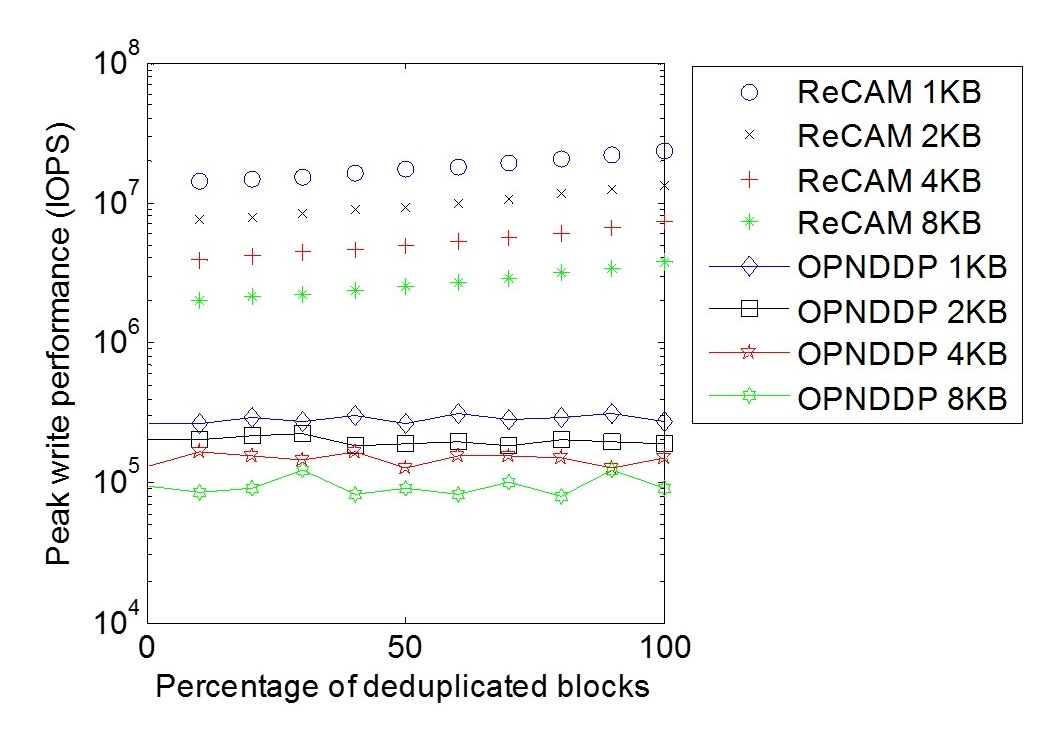
\includegraphics[scale=1]{Figures/dedup_perf.jpg}}
	\caption{Write performance for different block sizes vs. percentage of deduplicated blocks, for data blocks of 1KB, 2KB, 4KB and 8KB (OPNDDP = Opendedup).}
	\label{fig:dedup_performance}
\end{figure}

\begin{figure}[h!]
	\centerline{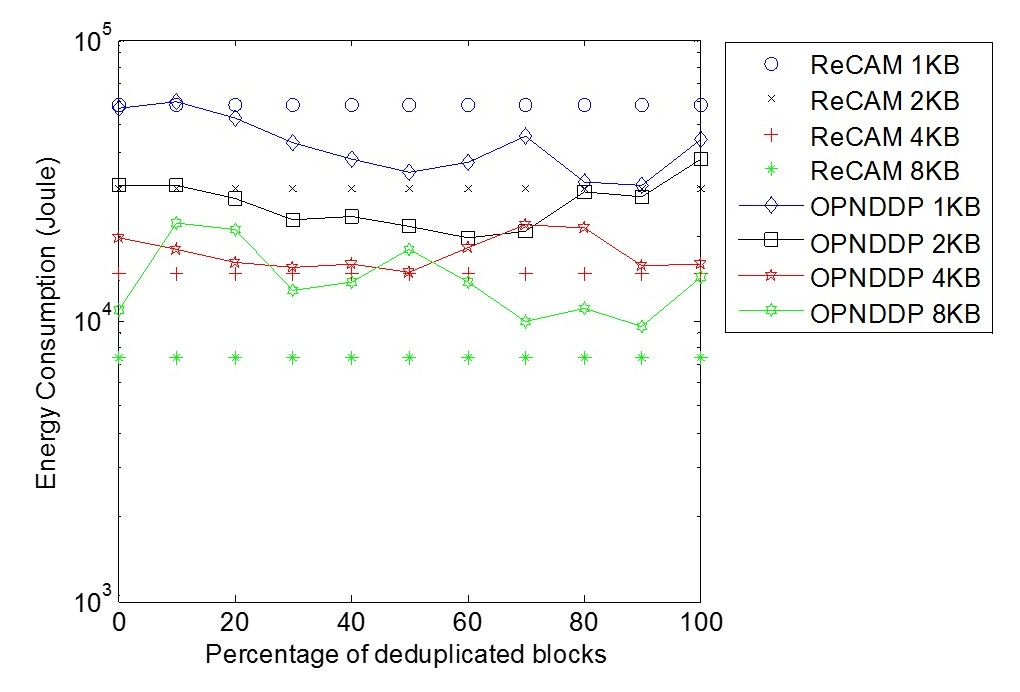
\includegraphics[scale=1]{Figures/dedup_energy.jpg}}
	\caption{Deduplication energy for different block sizes vs. percentage of deduplicated blocks, for data blocks of 1KB, 2KB, 4KB and 8KB while writing 50GByte of data.}
	\label{fig:dedup_energy}
\end{figure}




\section{Conclusions}

Near-data processing-in-storage is inherently limited because it is based on replicating von Neumann processors near storage. Therefore, it potentially faces some of von Neumann architecture problems, such as the bandwidth wall. To resolve this problem and allow for full utilization of ultra-high internal bandwidth of future resistive memory based SSD, we propose a novel in-data processing-in-storage architecture based on Resistive Content Addressable Memory (ReCAM). Unlike near-data in-SSD processing, ReCAM enables storage with in-data associative processing capabilities. It can contain hundreds of millions of data rows, each row serving as an associative processing unit. ReCAM requires no in-storage processing cores external to the storage arrays. There is no data transfer outside the storage arrays. Therefore, the internal bandwidth of the resistive memory based storage can be utilized to its fullest extent, considerably improving computation throughput of processing-in-storage system.
The ReCAM architecture, capable of general purpose associative processing, has been applied to a variety of challenging data and compute intensive problems, such as various machine learning and bioinformatics algorithms. The paper investigated SpMV, K-Means, KNN and Smith-Waterman sequence alignment algorithms and compared RCAM to other published analyses. 


\bibliography{example}

%\received{July, 2017}

\end{document}
